\documentclass[12pt, a4paper, oneside]{ctexart}
\usepackage{amsmath, amsthm, amssymb, bm, color, framed, graphicx, hyperref, mathrsfs, geometry}
\usepackage{algorithm, algorithmicx, algpseudocode}
\usepackage{caption, subcaption}

\title{\textbf{机器学习第四次作业}}
\author{汪隽立\ 2021012957}
\date{\today}
\linespread{1.5}
\definecolor{shadecolor}{RGB}{241, 241, 255}
\newcounter{problemname}
\newenvironment{problem}[1]{\begin{shaded}\par\noindent\textbf{题目 #1. }}{\end{shaded}\par}
\newenvironment{solution}[1]{\par\noindent\textbf{解答 #1. }\par}{\par}
\newenvironment{note}{\par\noindent\textbf{题目\arabic{problemname}的注记. }}{\par}

\geometry{a4paper,scale=0.8}
\begin{document}

\maketitle

\begin{solution}{2.1}
    \begin{equation}
        V^{\pi}(s) = \mathbb{E}_{\pi} \left[ \sum_{\tau=0}^{\infty} \gamma^\tau R_{t+\tau+1} \bigg| S_t = s \right] \nonumber
    \end{equation}
\end{solution}

\begin{solution}{2.2}
    \begin{equation}
        V^{\pi}(s) = \mathbb{E}_{\pi} \left[ R_{t+1}+\gamma V^{\pi}(S_{t+1})\bigg| S_t=s \right] \nonumber
    \end{equation}
\end{solution}

\begin{solution}{2.3}
    \begin{align}
        V_1^{\pi_0}(A)&=-4+\gamma V_0^{\pi_0}(B)=-4 \nonumber \\
        V_1^{\pi_0}(B)&=\frac{1}{2}\times(1+\gamma V_0^{\pi_0}(A))+\frac{1}{2}\times(2+\gamma V_0^{\pi_0}(C))=1.5 \nonumber \\ 
        V_1^{\pi_0}(C)&=\frac{1}{2}\times(8+\gamma (\frac{1}{4}V_0^{\pi_0}(C)+\frac{3}{4}V_0^{\pi_0}(A)))+\frac{1}{2}\times(0+\gamma V_0^{\pi_0}(B))=4 \nonumber
    \end{align}
\end{solution}

\begin{solution}{2.4}
    \begin{align}
        q_{\pi_0}(B,ba)&=1+\gamma V_1^{\pi_0}(A) = -1 \nonumber \\
        q_{\pi_0}(B,bc)&=2+\gamma V_1^{\pi_0}(C) = 4 \nonumber \\
        q_{\pi_0}(C,ca)&=8+\gamma (\frac{1}{4}V_1^{\pi_0}(C) + \frac{3}{4}V_1^{\pi_0}(A)) = 7 \nonumber \\
        q_{\pi_0}(C,cb)&=0+\gamma V_1^{\pi_0}(B) = 0.75 \nonumber
    \end{align}
    故更新后,$\pi_1(A)=ab$, $\pi_1(B)=bc$, $\pi_1(C)=ca$.
\end{solution}

\begin{solution}{3.1}
    \begin{align}
        V(A)=\frac{1}{2}(0+2)&=1 \nonumber \\
        V(B)=\frac{1}{2}(-2-3)&=-\frac{5}{2} \nonumber \\ 
        Q(A,a)=\frac{1}{2}(0+2)&=1 \nonumber \\
        Q(B,b)=\frac{1}{2}(-2-3)&=-\frac{5}{2} \nonumber
    \end{align}
\end{solution}

\begin{solution}{3.2}
    \begin{align}
        V(A)=\frac{1}{4}(0+2-3+1)&=0 \nonumber \\
        V(B)=\frac{1}{4}(-2-3-3-3)&=-\frac{11}{4} \nonumber \\ 
        Q(A,a)=\frac{1}{4}(0+2-3+1)&=0 \nonumber \\
        Q(B,b)=\frac{1}{4}(-2-3-3-3)&=-\frac{11}{4} \nonumber
    \end{align}
\end{solution}

\begin{solution}{3.3}
    在初始时,$V(A)=V(B)=0$, $Q(A,a)=Q(B,b)=0$。$V$的迭代过程如下:
    \begin{align}
        V(B)=0.1\times(-2)&=-0.2 \nonumber \\
        V(A)=0.1\times(3+V(B))&=0.28 \nonumber \\
        V(B)=0.9\times(-0.2)+0.1\times(-3+0)&=-0.48 \nonumber \\
        V(A)=0.9\times(0.28)+0.1\times(3+V(A))&=0.58 \nonumber \\
        V(A)=0.9\times(0.58)+0.1\times(2+V(B))&=0.674 \nonumber \\
        V(B)=0.9\times(-0.48)+0.1\times(-4+V(A))&=-0.7646 \nonumber \\
        V(A)=0.9\times(0.674)+0.1\times(4+V(B))&=0.93014 \nonumber \\
        V(B)=0.9\times(-0.7646)+0.1\times(-3+0)&=-0.98814 \nonumber
    \end{align}
    于是我们得到$V(A)=0.93014$, $V(B)=-0.98814$。因为整个过程中在状态$A$, $B$分别只采取了策略$a$, $b$,故$Q(A, a)=V(A)=0.93014$,$Q(B, b)=V(B)=-0.98814$.
\end{solution}

\begin{solution}{4.3}
    \begin{table}[htbp]
        \centering
        \begin{tabular}{|c|c|c|}
            \hline
            \textbf{Learning Rate} & \textbf{Average Reward} & \textbf{Average Moves} \\
            \hline
            $0.01$ & $-177.645$ & $179.85$ \\
            \hline
            $0.1$ & $8.03$ & $12.97$ \\
            \hline
            $1$ & $7.565$ & $13.435$ \\
            \hline
            $2$ & $-200.0$ & $200.0$ \\
            \hline
        \end{tabular}
        \caption{不同学习率下Q\_Learning的表现}
        \label{tab:qlearning}
    \end{table}

    \begin{table}[htbp]
        \centering
        \begin{tabular}{|c|c|c|}
            \hline
            \textbf{Learning Rate} & \textbf{Average Reward} & \textbf{Average Moves} \\
            \hline
            $0.01$ & $-179.78$ & $181.775$ \\
            \hline
            $0.1$ & $7.955$ & $13.045$ \\
            \hline
            $1$ & $7.625$ & $13.435$ \\
            \hline
            $2$ & $-200.0$ & $200.0$ \\
            \hline
        \end{tabular}
        \caption{不同学习率下SARSA的表现}
        \label{tab:sarsa}
    \end{table}

    实验结果见表 \ref{tab:qlearning}和表 \ref{tab:sarsa}。可以看出,对Q\_Learning和Sarsa而言,最佳的学习率都为$0.1$,过高和过低的学习率会导致模型没有学习能力/损失函数震荡。\par
    
    另外,可以看出Q\_Learning和Sarsa都对学习率呈现了一定的鲁棒性,当学习率在$0.1$至$1$之间时,模型的表现都比较稳定。
\end{solution}

\begin{solution}{4.4}
    \begin{figure}
        \centering
        \includegraphics[width=0.8\textwidth]{../code/sarsa_Q_learning/figs/Q_Learning with lr=0.1.png}
        \caption{Q\_Learning with lr=0.1}
        \label{fig:qlearning}
    \end{figure}

    \begin{figure}
        \centering
        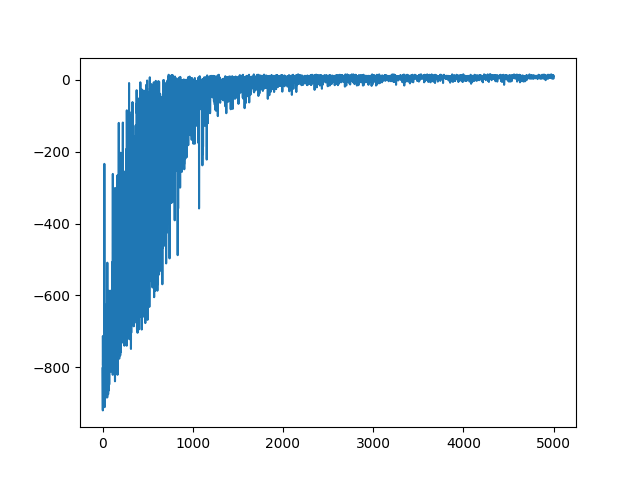
\includegraphics[width=0.8\textwidth]{../code/sarsa_Q_learning/figs/Sarsa with lr=0.1.png}
        \caption{Sarsa with lr=0.1}
        \label{fig:sarsa}
    \end{figure}

    实验结果如 \ref{fig:qlearning}和 \ref{fig:sarsa}所示。可以看出 Sarsa 相较于 Q\_Learning 而言更稳定。\par

    除此以外,观察实验框架给出的设定可知,初始时$\epsilon$-Greedy算法的$\epsilon=1$,而随着学习的进行,$\epsilon$会慢慢降低。这可能导致的结果是,在 Sarsa 算法中,由于初始的$\epsilon$过高,在更新$Q(s,a)$时完全基于随机策略。故 Sarsa 的收敛性很可能受到前几次随机采样的影响。一个可以改进的地方是,可以将初始的$\epsilon$适当调小,以平衡探索与利用在算法中的作用。
\end{solution}

\begin{solution}{5.3}
    \begin{figure}[htbp]

        \centering
        \begin{minipage}[t]{0.48\textwidth}
        \centering
        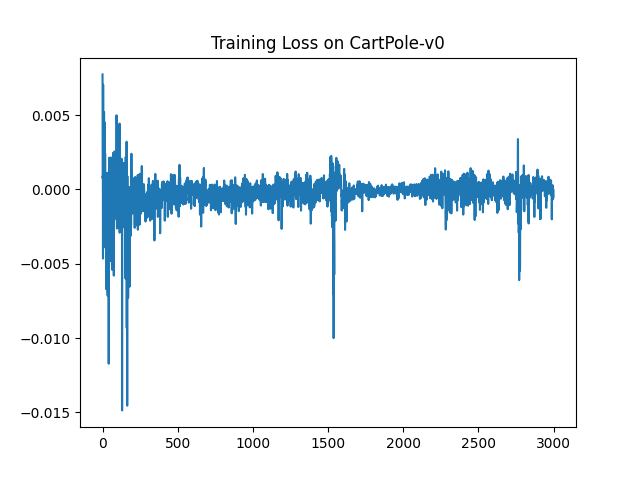
\includegraphics[width=5cm]{../code/policy_gradient/figs/Training Loss on CartPole-v0 with algorithm TDActorCritic .png}
        \caption{TDActorCritic 在 CartPole-v0 上的训练损失}
        \end{minipage}
        \begin{minipage}[t]{0.48\textwidth}
        \centering
        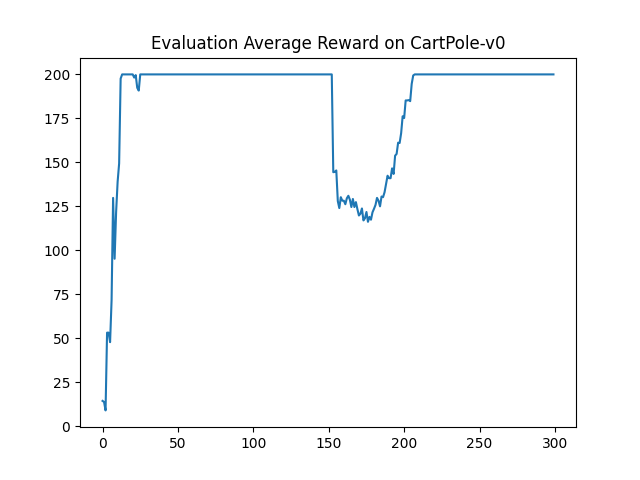
\includegraphics[width=5cm]{../code/policy_gradient/figs/Evaluation Average Reward on CartPole-v0 with algorithm TDActorCritic.png}
        \caption{TDActorCritic 在 CartPole-v0 上的平均奖励}
        \end{minipage}

    \end{figure}

    \begin{figure}[htbp]

        \centering
        \begin{minipage}[t]{0.48\textwidth}
        \centering
        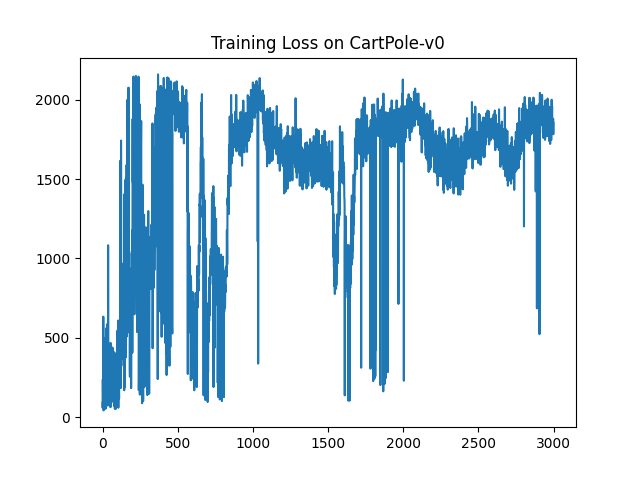
\includegraphics[width=5cm]{../code/policy_gradient/figs/Training Loss on CartPole-v0 with algorithm REINFORCE .png}
        \caption{REINFORCE 在 CartPole-v0 上的训练损失}
        \end{minipage}
        \begin{minipage}[t]{0.48\textwidth}
        \centering
        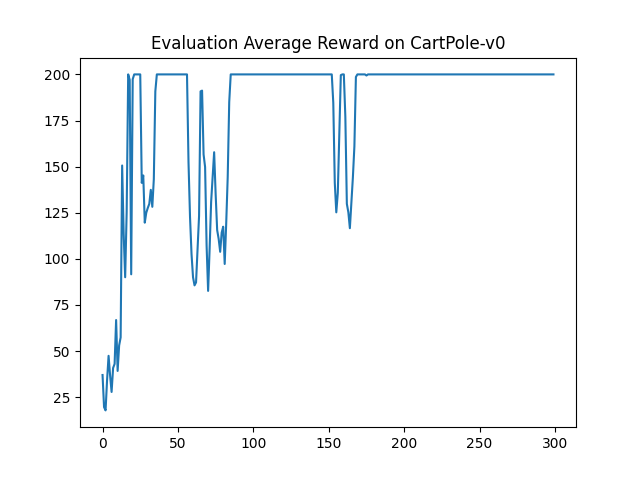
\includegraphics[width=5cm]{../code/policy_gradient/figs/Evaluation Average Reward on CartPole-v0 with algorithm REINFORCE.png}
        \caption{REINFORCE 在 CartPole-v0 上的平均奖励}
        \end{minipage}

    \end{figure}

    \begin{figure}[htbp]

        \centering
        \begin{minipage}[t]{0.48\textwidth}
        \centering
        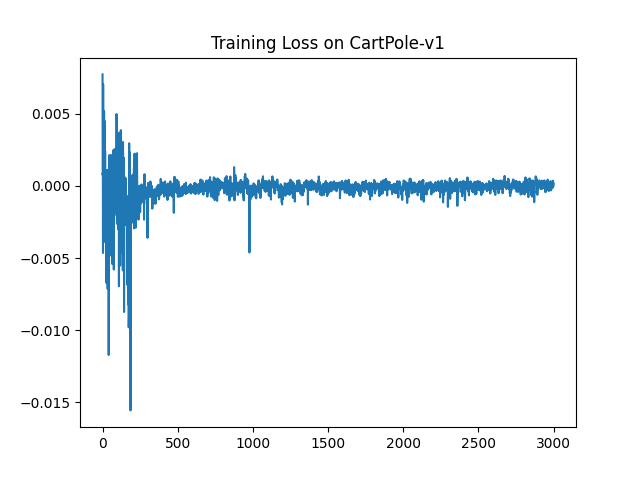
\includegraphics[width=5cm]{../code/policy_gradient/figs/Training Loss on CartPole-v1 with algorithm TDActorCritic .png}
        \caption{TDActorCritic 在 CartPole-v1 上的训练损失}
        \end{minipage}
        \begin{minipage}[t]{0.48\textwidth}
        \centering
        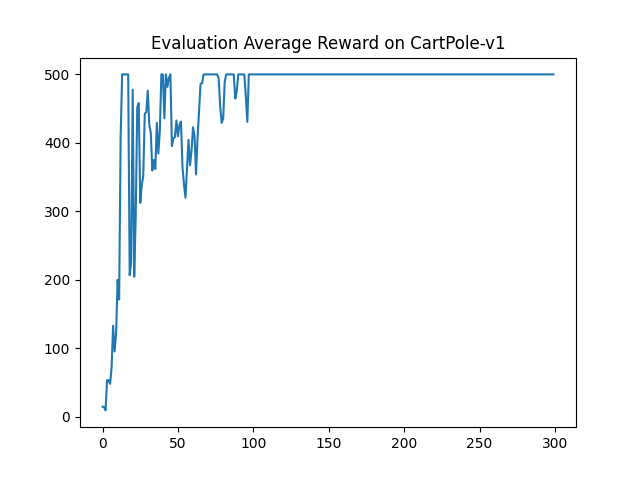
\includegraphics[width=5cm]{../code/policy_gradient/figs/Evaluation Average Reward on CartPole-v1 with algorithm TDActorCritic.png}
        \caption{TDActorCritic 在 CartPole-v1 上的平均奖励}
        \end{minipage}

    \end{figure}

    \begin{figure}[htbp]

        \centering
        \begin{minipage}[t]{0.48\textwidth}
        \centering
        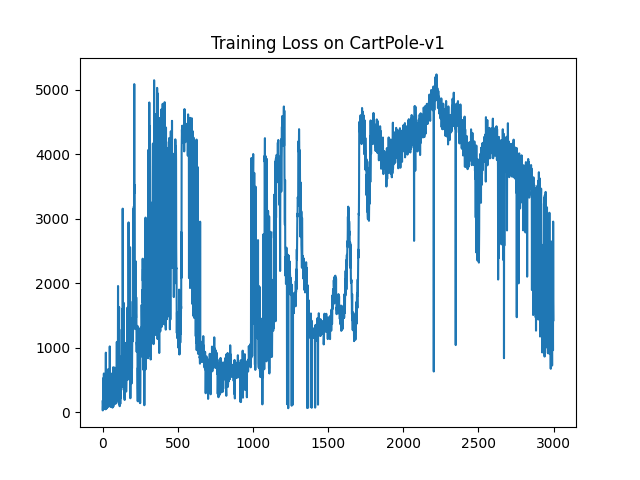
\includegraphics[width=5cm]{../code/policy_gradient/figs/Training Loss on CartPole-v1 with algorithm REINFORCE .png}
        \caption{REINFORCE 在 CartPole-v1 上的训练损失}
        \end{minipage}
        \begin{minipage}[t]{0.48\textwidth}
        \centering
        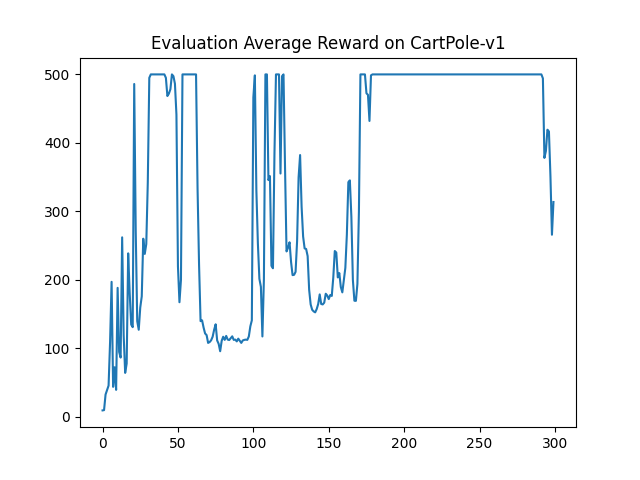
\includegraphics[width=5cm]{../code/policy_gradient/figs/Evaluation Average Reward on CartPole-v1 with algorithm REINFORCE.png}
        \caption{REINFORCE 在 CartPole-v1 上的平均奖励}
        \end{minipage}

    \end{figure}

    实验结果如图所示。AC 在 CartPole-v0 和 CartPole-v1 上均取得了最佳的平均奖励,而 REINFORCE 则有一些抖动。\par
    可以明显地看出 TDActorCritic 相较于 REINFORCE 有更好的稳定性与收敛速率。这是因为, TDActorCritic 是基于 TD 的一步采样,拥有更小的方差。\par
    除此以外,TDActorCritic 还展现了更好的鲁棒性。在 CartPole-v0 实验中,即使某一时刻偏离了最佳策略,TDActorCritic 也能迅速恢复到最佳策略上去。
\end{solution}

\end{document}